\chapter{Band structures of crystals}
\section{Energy band structures at $T = 0K$}
As it turns out, as mentioned in the previous chapter (chapter \ref{ch:crystals}), the behaviour of the crystal can be represened by just a few important energy bands. In this section, we start with a simple case: the band structure of a semiconductor/insulator in 1D, see figure \ref{fig:simple_bandstruct}. As it turns out, only the valence band (VB) and conduction band (CB) (in the neighbourhood of the $\Gamma$-point) are needed to obtain all information about the behaviour of the electrons. \\ \par
As we see, the further we go away from the $\Gamma$-point (thus increasing/decreasing $k$), the more the $E_g$ becomes. Meaning thermally exiting electrons is becomes more difficult. That's why the $\Gamma$-point is so important. These electrons can be described as quasi-particles, that means free-electrons. As we will see, something will happen to the mass of the electrons. \\ \par
First, we look at the conduction band. Because we are only interested in the electrons near the $\Gamma$-point, we can use a taylor expansion for the description of the energy:
\begin{align}
	E_{CB}(k) &\approx E_{CB}(0) + \left\frac{dE_{CB}}{dk}\right|_{k=0}k + \frac{1}{2}\left\frac{d^2E_{CB}}{dk^2}\right|_{k=0}k^2 \\
	&= E_{CB}(0) + \frac{1}{2}\left\frac{d^2E_{CB}}{d^2k}\right|_{k=0}k^2
\end{align}
Then for a free electron we know that:
\begin{equation}
	E^{(0)}(k) = \frac{\hbar^2k^2}{2m}
\end{equation}
Then if we use the following substitution:
\begin{equation}
	\frac{1}{2}\left\frac{d^2E_{CB}}{dk^2}\right|_{k=0} = \frac{\hbar^2}{2m^{*}} \iff m^{*} = \hbar^2\left(\left\frac{d^2E_{CB}}{d^2k}\right|_{k=0}\right)^{-1}
\end{equation}
We get a similar expresion to the energy of a free electron:
\begin{equation}
	E_{CB}(k) = E_{CB}(0) + \frac{\hbar^2}{2m^{*}}k^2
\end{equation}
Except, now the mass is different. This mass is called the effective mass. We can conclude that the electrons in the CB, near the $\Gamma$-point, behave as a free electron, albeit they have a different mass. \\ \par
A similar derivation for the VB can be made, we can just substitute $E_{CB}$ by $E_{VB}$. As you might notice, the VB and CB don't need to be the same and therefore, the $m^{*}$ isn't necessary the same. \nt{Notice that the effective mass for the VB is smaller than zero. How do we define that? See section \ref{sec:holes}}

\begin{figure}
	\centering
	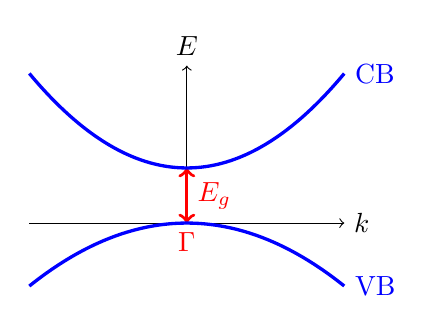
\begin{tikzpicture}[domain=-2:2]
		\draw[->, black]	(-2, 0) to (2, 0) node[right]{$k$};
		\draw[->, black]	(0, 0) to (0, 2) node[above]{$E$};

		\draw[red] 			(0, 0) node[below]{$\Gamma$};

		\draw[<->, red, very thick]	(0, 0) to node[right]{$E_g$} (0, 0.7);

		\draw[blue, very thick] plot[samples=200] (\x, 0.3*\x*\x + 0.7) node[right]{CB};
		\draw[blue, very thick] plot[samples=200] (\x, -0.2*\x*\x) node[right]{VB};
	\end{tikzpicture}
	\caption{A simple 1D semiconductor/insulator band structure}
	\label{fig:simple_bandstruct}
\end{figure}

\subsection{Generalization of the energy band structure at 0K}
In general we can say that the energy dispersion is the following:
\begin{equation}
	E_n(\vec{k}) \approx E_n(\vec{k}_0) + \frac{1}{2}\sum_{i, j}^{}\left\frac{\delta^2E}{\delta k_i \delta k_j}\right|_{\vec{k} = \vec{k}_0}(k_i - k_{i0})(k_j - k_{j0}) \qquad \text{for } j, i = 1, 2, 3
\end{equation}
We then define the effective mass as:
\begin{equation}
	\left[m^{*}_{i, j}\right]^{-1} = \frac{1}{\hbar^2}\left\frac{\delta^2 E_n(\vec{k})}{\delta k_i \delta k_j}\right|_{\vec{k} = \vec{k}_0}
\end{equation}
The effective mass can be written as a matrix/tensor, this matrix/tensor is symmetric. Furhtermore, it is always possible to coordinate transformation $k_1$, $k_2$, $k_3$ to $k'_1$, $k'_2$, $k'_3$ in order that the matrix becomes a diagonal matrix. \\ \par
After diagonalization, the matrix can be simplified to:
\begin{equation}
	\left[
		\begin{array}{ccc}
			\frac{1}{m_1^{*}} & 0 & 0 \\
			0 & \frac{1}{m_2^{*}} & 0 \\
			0 & 0 & \frac{1}{m_3^{*}}
		\end{array}
	\right]
	=
	\left[
		\begin{array}{ccc}
			\left\frac{\delta^2 E_n(\vec{k})}{\delta k_1^2}\right|_{\vec{k} = \vec{k}_0} & 0 & 0 \\
			0 & \left\frac{\delta^2 E_n(\vec{k})}{\delta k_2^2}\right|_{\vec{k} = \vec{k}_0} & 0 \\
			0 & 0 & \left\frac{\delta^2 E_n(\vec{k})}{\delta k_3^2}\right|_{\vec{k} = \vec{k}_0}
		\end{array}
	\right]
\end{equation}
What we can conclude from this is that if we find the right coordinate transformation then the effective mass of the electron can be different in every direction.

\subsection{Some examples}
\ex{3D example 1}{
	Suppose you have a semiconductor where the CB minimum is located at the $\Gamma$-point. This semiconductor is isotropic, meaning it has $m_x^{*} = m_y^{*} = m_z^{*} = m^{*}$. In this case take $m^{*} > 0$. \\
	In this case we can define $E_n(\vec{k})$ as:
	\begin{equation}
		E_n(\vec{k}) = E_n(\vec{0}) + \frac{\hbar^2}{2}\left[\frac{k_x^2}{2m_x^*} + \frac{k_y^2}{2m_y^*} + \frac{k_z^2}{2m_z^*}\right] = E_n(\vec{0}) + \frac{\hbar^2}{2m^*}k^2 \text{with } k^2 = k^2_x + k^2_y + k^2_z
	\end{equation}
	For any value of energy $E > E_n(\vec{0})$, we can define constant energy surfaces that define a sphere with radius
	\begin{equation}
		R = \sqrt{(E-E_n(\vec{0}))\frac{2m^*}{\hbar^2}}
	\end{equation} \\ \par
	When we now look at the VB maximum, we have a problem: $m^* < 0$. This problem is resolved by introducing $m^*_h = -m^*$, this is explain in section \ref{sec:holes}.
}

\ex{Multiple bands}{
	In the picture are the so-called 'split off', 'light holes', 'heavy holes' displayed. Because the curvature determines the effective mass, a wider curve means a heavier hole. Note that we speak about holes and not electrons anymore. The according energy dispersion functions are:
	\begin{align}
		E_{heavy hole} &= \frac{\hbar^2}{2m^*_{hh}}(k_x^2 + k_y^2 + k_z^2) \\
		E_{light hole} &= \frac{\hbar^2}{2m^*_{lh}}(k_x^2 + k_y^2 + k_z^2) \\
		E_{split off} &= \frac{\hbar^2}{2m^*_{so}}(k_x^2 + k_y^2 + k_z^2)
	\end{align}
	Notice that we introduced the hole effective mass and added a - sign to compensate for the change of variable.
	\begin{center}
		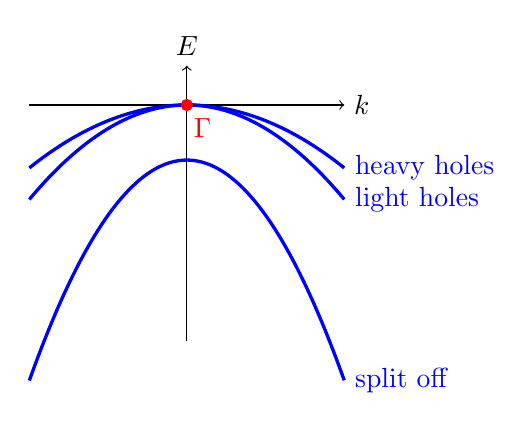
\begin{tikzpicture}[domain=-2:2]
			\draw[->, black]	(-2, 0) to (2, 0) node[right]{$k$};
			\draw[->, black]	(0, -3) to (0, 0.5) node[above]{$E$};

			\draw[blue, very thick] plot[samples=200] (\x, -0.7*\x*\x - 0.7) node[right]{split off};
			\draw[blue, very thick] plot[samples=200] (\x, -0.3*\x*\x) node[right]{light holes};
			\draw[blue, very thick] plot[samples=200] (\x, -0.2*\x*\x) node[right]{heavy holes};

			\filldraw[red] 		(0, 0) circle (2pt);
			\draw[red]			(0.2, -0.05) node[below]{$\Gamma$};
		\end{tikzpicture}
	\end{center}
}

\ex{Indirect semiconductor}{
	These semiconductors have, typically, a non-isotropic effetive mass tensor. If we take Si for example, we get the following minima for the conduction band (denoted in red on the figure). These points come just before the $X$-point (like a $\Gamma$-point) the first Brouillin Zone.
	\begin{center}
		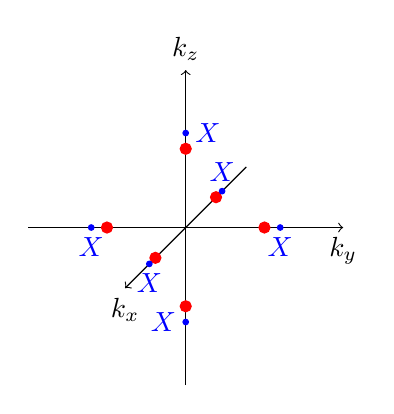
\begin{tikzpicture}
			\draw[->, black]	(-2, 0, 0) to (2, 0, 0) node[below]{$k_y$};
			\draw[->, black]	(0, -2, 0) to (0, 2, 0) node[above]{$k_z$};
			\draw[->, black]	(0, 0, -2) to (0, 0, 2) node[below]{$k_x$};

			\filldraw[red]		(-1, 0, 0) circle (2pt)
								(1, 0, 0) circle (2pt)
								(0, -1, 0) circle (2pt)
								(0, 1, 0) circle (2pt)
								(0, 0, -1) circle (2pt)
								(0, 0, 1) circle (2pt);

			\filldraw[blue]		(-1.2, 0, 0) circle (1pt) node[below]{$X$}
								(1.2, 0, 0) circle (1pt) node[below]{$X$}
								(0, -1.2, 0) circle (1pt) node[left]{$X$}
								(0, 1.2, 0) circle (1pt) node[right]{$X$}
								(0, 0, -1.2) circle (1pt) node[above]{$X$}
								(0, 0, 1.2) circle (1pt) node[below]{$X$};
		\end{tikzpicture}
	\end{center}
	Then the energy dispersion formula will become (in function of $\alpha = 1, 2, 3, 4, 5, 6$, one for each minimum):
	\begin{equation}
		E_{\alpha}(\vec{k}) = E_{\alpha} + \frac{\hbar^2}{2}\left[\frac{(k_x - k_{0, \alpha, x})^2}{m^*_{\alpha, x}} + \frac{(k_y - k_{0, \alpha, y})^2}{m^*_{\alpha, y}} + \frac{(k_z - k_{0, \alpha, z})^2}{m^*_{\alpha, z}}\right]
	\end{equation}
	We also immediatly see that for the effective inverse mass tensor, alle non-diagonal elements are zero, resulting in:
	\begin{equation}
		\left[m^*_{ij}\right]^{-1} = \left[
		\begin{array}{ccc}
			\frac{1}{m^*_{\alpha, x}} & 0 & 0 \\
			0 & \frac{1}{m^*_{\alpha, y}} & 0 \\
			0 & 0 & \frac{1}{m^*_{\alpha, z}}\\
		\end{array}
		\right]
	\end{equation}
	As it turns out, there is some symmetry in the effective masses along different axes:\\
	\quad the effective masses along the $k_x$-axis give: $m^*_{\alpha, x} = m^*_l$ and $m^*_{\alpha, y} = m^*_{\alpha, z} = m^*_t$, \\
	\quad the effective masses along the $k_y$-axis give: $m^*_{\alpha, y} = m^*_l$ and $m^*_{\alpha, x} = m^*_{\alpha, z} = m^*_t$, \\
	\quad the effective masses along the $k_z$-axis give: $m^*_{\alpha, z} = m^*_l$ and $m^*_{\alpha, x} = m^*_{\alpha, y} = m^*_t$. \\ \newline
	\textbf{What surfaces do we get now?} \\
	The energy dispersion diagram we get for $\alpha = 1$ and $E > E_1(\vec{k}_{0, 1})$ is:
	\begin{equation}
		E_{1}(\vec{k}) = E_{1} + \frac{\hbar^2}{2}\left[\frac{(k_x - k_{0, 1, x})^2}{m^*_l} + \frac{(k_y - k_{0, 1, y})^2}{m^*_t} + \frac{(k_z - k_{0, 1, z})^2}{m^*_t}\right]
	\end{equation}
	This gives us an ellipsoidal surface. In the 3D space, we will see small elongated ellipsoids along the axes.
}
\ex{Intermezzo: Ge} {
	If we now look at Ge, we get the CB minimum at the $L$-points which are in the [1 1 1] direction. If we choose a normal axes orientation ($k_x = $ [1 0 0], etc.). We get ellipsoids along the [1 1 1] (and the two axes perpendicular to it) axis. This means the effective mass tensor will have a contribution of all elements of the tensor, it will not be a diagonal matrix. Rotate the coordinate system accordingly!
}

\section{Energy band structures at $T > 0K$}
At a finite temperature there is a chance electrons are excited from the VB to the CB. We can say that there is a probability a certain E-state is occupied. Because particles can be defined in two ways in Quantum mechanics, we will separate them here, too.

\subsection{Bosons - integer spin}
For bosons, any energy state $E_i$ can be occupied by an unlimited amount of particles. The probability distribution is given by the Bose-Einstein distribution:
\begin{equation}
	f(E) = \frac{1}{e^{\beta E} - 1} \quad \text{with } \beta = \frac{1}{k_BT}
\end{equation}
We will not further discuss this case.

\subsection{Fermions - half integer spin}
Every energy state can be occupied by at most one particle. this is called the \textbf{Pauli exlusion principle}. Still, one has to pay attention to degeneracies. For electrons, one energy state has two degeneracies. The probability distribution is give by the Fermi-Dirac distribution, also given in figure \ref{fig:fermidiracdistr}:
\begin{equation}
	f(E) = \frac{1}{1 - e^{\beta (E - \mu)}} \quad \text{with } \beta = \frac{1}{k_BT} \text{ and } \mu = \text{ the chemical potential ($E_g$ for intrinsic semiconductor)} \label{eqn:elec_fermi-dirac}
\end{equation}
What is the physical significane of this distribution function? Well, $f(E) = $ probability to occupy a state at energy E. Meaning that $1 - f(E) = $ probability that a state E is not occupied.
\begin{figure}[h]
	\centering
	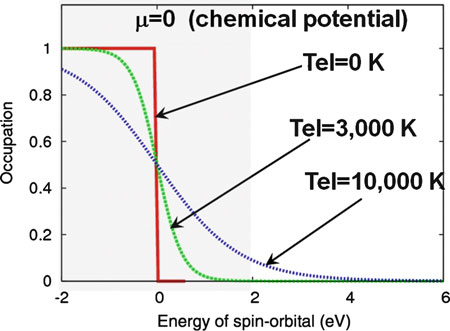
\includegraphics[scale=0.5]{./fermi.png}
	\caption{The Fermi-Dirac distribution for different temperatures}
	\label{fig:fermidiracdistr}
\end{figure}
As we know, for $\beta\mu >> 1$ we can use the Maxwell-Botzmann distribution. \\ \par
When graphing the Fermi-Dirac distribution in a band diagram, we get the following graph for different temperatures, see figure \ref{fig:fermidiracinenergyband}.
\begin{figure}[h]
	\centering
	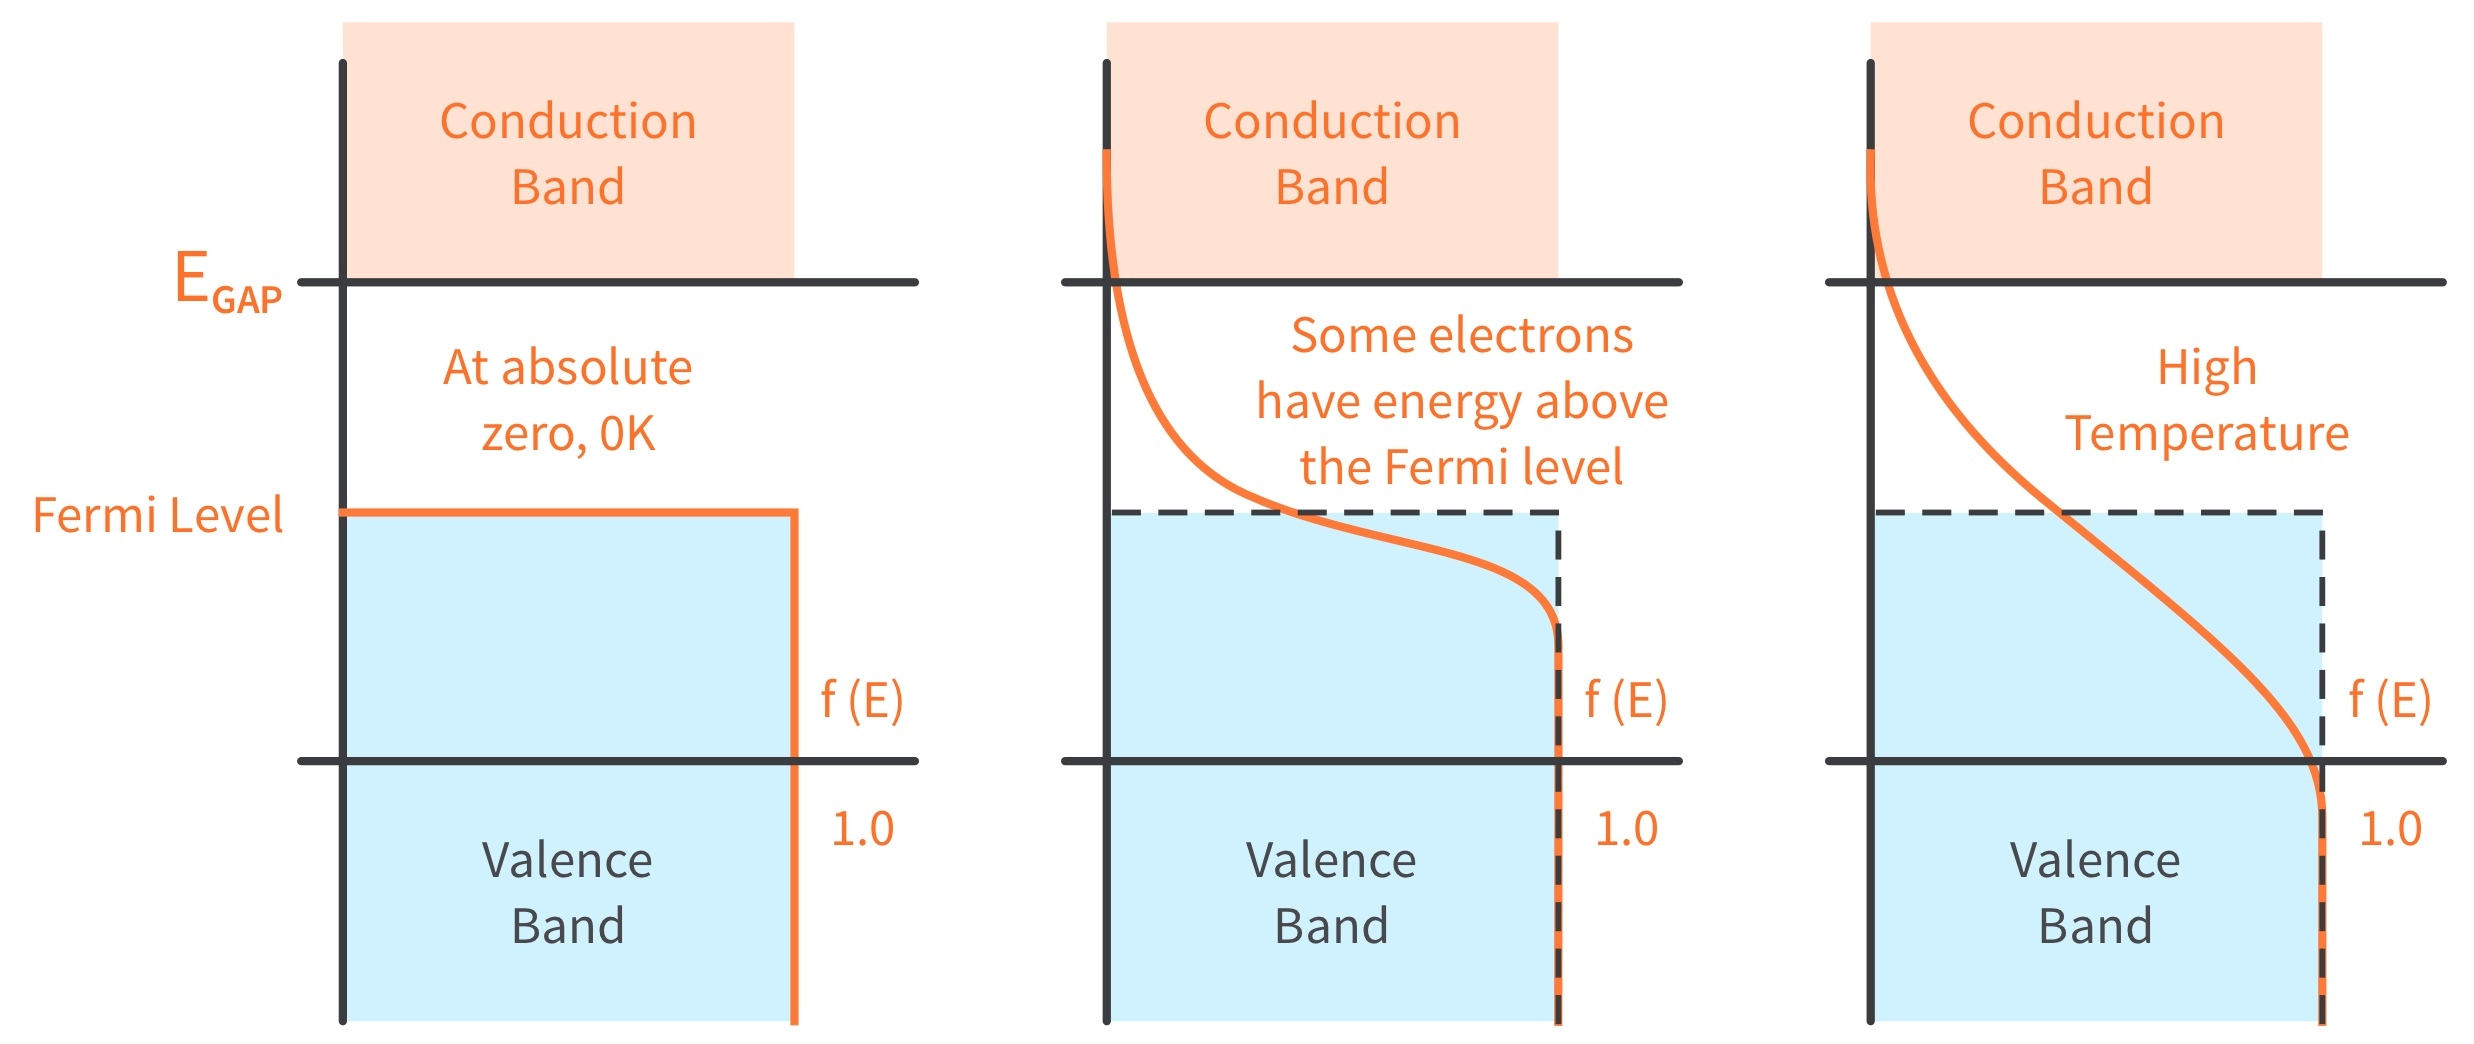
\includegraphics[scale=0.2]{./fermidirac_in_banddiagram.jpg}
	\caption{The Fermi-Dirac distribution for different temperatures}
	\label{fig:fermidiracinenergyband}
\end{figure}
\nt{The reason for having the Fermi-Dirac function going to 1 is that it is an electron is a fermion and only one can occupy a state.}
